%% SECTION 4.4 %%
\section{The VC Inequality}
\label{sec: VC inequality}

We have now introduced all the concepts required to formulate the main result of this chapter: the VC inequality.

\begin{theorem}[VC Inequality]
\label{thm: VC inequality}
For $n > 2 V_{\mathcal{A}}$, every family of sets $\mathcal{A}$ satisfies
\[
    \Exp[\sup_{A \in \mathcal{A}} \abs{\mu_n(A) - \mu(A)}] \leq 2 \sqrt{\frac{2 V_{\mathcal{A}} \log(2\e n / V_{\mathcal{A}})}{n}}.
\]
\end{theorem}

We split the proof of this result into three steps:

\begin{enumerate}
    \item Using symmetrization, we prove that
    \[
        \Exp[\sup_{A \in \mathcal{A}} \abs{\mu_n(A) - \mu(A)}] \leq 2 \mathfrak{R}_n(\mathcal{A}).
    \]
    Note that this is precisely the bound \eqref{eq: symmetrization bound} obtained in Section \ref{sec: symmetrization}.

    \item We bound the Rademacher complexity of $\mathcal{A}$ using shatter coefficients:
    \[
        \mathfrak{R}_n(\mathcal{A}) \leq \sqrt{\frac{2 \log(2 \mathcal{S}_{\mathcal{A}}(n))}{n}}.
    \]

    \item Finally, for $n > 2 V_{\mathcal{A}}$, we bound the shatter coefficients $\mathcal{S}_{\mathcal{A}}(n)$ of $\mathcal{A}$ by
    \[
        \mathcal{S}_{\mathcal{A}}(n) \leq \left(\frac{\e n}{V_{\mathcal{A}}}\right)^{V_{\mathcal{A}}},
    \]
    which is a result known as the \emph{Sauer-Shelah} lemma.
\end{enumerate}

Since the first step is already done, let's tackle step number 2. As an intermediate result, we prove a bound of the Rademacher complexity of finite subsets in $\R^n$. This will turn out to be immensely useful, as we can express the Rademacher complexity of a family of sets $\mathcal{A}$ in terms of the Rademacher complexity of finite subsets in $\R^n$, i.e., $\mathfrak{R}_n(\mathcal{A}) = \sup_{z \in \mathcal{Z}^n} \mathfrak{R}_n(T(z))$, where $T(z)$ is defined as in \eqref{eq: T(z)}.

\begin{lemma}
\label{lem: bound on rademacher complexity of finite set}
For a \emph{finite} set $B \subset \R^n$, it holds
\[
    \mathfrak{R}_n(B) \leq \max_{b \in B} \norm{b}_2 \frac{\sqrt{2 \log(2 \abs{B})}}{n},
\]
where $\norm{\cdot}_2$ denotes the Euclidean norm on $\R^d$.
\end{lemma}

\begin{proof}
By definition,
\[
    n \mathfrak{R}_n(B) = \Exp[\max_{b \in B} \abs{Z_b}],
\]
where $Z_b = \sum_{i=1}^n \sigma_i b_i$. Since $-\abs{b_i} \leq \sigma_i b_i \leq \abs{b_i}$ holds almost surely, Hoeffding's lemma (Lemma \ref{lem: hoeffding}) bounds the moment generating function of $Z_b$ by
\begin{equation}
\label{eq: proof of bound on rademacher complexity of finite set}
    \Exp[\exp(s Z_b)] = \prod_{i=1}^n \Exp[\exp(s \sigma_i b_i)] \leq \prod_{i=1}^n \exp(s^2 b_i^2 / 2) = \operatorname{exp}(s^2 \norm{b}_2^2 / 2).
\end{equation}
To bound the quantity $\Exp[\max_{b \in B} \abs{Z_b}]$ we are interested in, let $\overline{B} = B \cup -B$, where $-B = \set{-b \with b \in B}$. For $s>0$,
\[
    \Exp[\max_{b \in B} \abs{Z_b}] = \Exp[\max_{b \in \overline{B}} Z_b] = s^{-1} \operatorname{log}(\operatorname{exp}(s \Exp[\max_{b \in \overline{B}} Z_b])) \leq s^{-1} \operatorname{log}({\color{blue} \Exp[\operatorname{exp}(s \max_{b \in \overline{B}} Z_b)]}),
\]
where the last inequality follows from Jensen's inequality applied to the function $x \mapsto \exp(sx)$. Since the logarithm is increasing, we can bound ${\color{blue} \Exp[\operatorname{exp}(s \max_{b \in \overline{B}} Z_b)]} \leq \sum_{b \in \overline{B}} \Exp[\exp(s Z_b)]$ to obtain
\begin{align*}
    \Exp[\max_{b \in B} \abs{Z_b}] &\leq s^{-1} \log(\sum_{b \in \overline{B}} \Exp[\exp(s Z_b)]) \leq s^{-1} \log(\sum_{b \in \overline{B}} \operatorname{exp}(s^2 \norm{b}_2^2 / 2) ) \\[4pt]
    &\leq \frac{\log(2 \abs{B})}{s} + \frac{s}{2} \max_{b \in B} \norm{b}_2^2 = \frac{2 \log(2 \abs{B}) + s^2 \max_{b \in B} \norm{b}_2^2}{2s},
\end{align*}
where the second inequality follows from \eqref{eq: proof of bound on rademacher complexity of finite set}, and the third inequality follows from the observation that $\max_{b \in \overline{B}} \norm{b}_2^2 = \max_{b \in B} \norm{b}_2^2$ and $\abs{\overline{B}} \leq 2 \abs{B}$. Optimizing the RHS over $s$ yields the optimal solution
\[
    s^* = \sqrt{\frac{2 \log(2 \abs{B})}{\max_{b \in B} \norm{b}_2^2}}.
\]
Plugging this back in yields the desired result, i.e.,
\[
    n \mathfrak{R}_n(B) = \Exp[\max_{b \in B} \abs{Z_b}] \leq \max_{b \in B} \norm{b}_2 \sqrt{2 \log(2 \abs{B})}. \qedhere
\]
\end{proof}

By applying the previous result to the finite set $T(z)$, we obtain
\[
    \mathfrak{R}_n(T(z)) \leq \max_{b \in T(z)} \norm{b}_2 \frac{\sqrt{2 \log(2 \abs{T(z)})}}{n}.
\]
Since each entry of a vector in $T(z)$ takes values in the set $\set{0, 1}$, we know that the Euclidean norm $\norm{b}_2$ of any vector $b \in T(z)$ is at most $\sqrt{n}$. Further, we know that the shatter coefficients $\mathcal{S}_{\mathcal{A}}(n)$ of $\mathcal{A}$ depend directly on the cardinality of the sets $T(z)$. Hence, the next result should come at no surprise.

\begin{proposition}
\label{prop: bound on rademacher complexity of family of sets}
For a family of sets $\mathcal{A}$, it holds
\[
    \mathfrak{R}_n(\mathcal{A}) \leq \sqrt{\frac{2 \log(2 \mathcal{S}_{\mathcal{A}}(n)) }{n}}.
\]
\end{proposition}

\begin{proof}
Observe that $\mathfrak{R}_n(\mathcal{A}) = \sup_z \mathfrak{R}_n(T(z))$, by Lemma \ref{lem: rademacher complexity of family of sets}, where $T(z)$ is defined as in \eqref{eq: T(z)}. Since $T(z) \subset \set{0, 1}^n$, we have $\norm{b}_2 \leq \sqrt{n}$ for all $b \in T(z)$ and all tuples $z = (z_1, \dots, z_n) \in \mathcal{Z}^n$. Hence, by Lemma \ref{lem: bound on rademacher complexity of finite set}, we have
\[
    \mathfrak{R}_n(\mathcal{A}) \leq \sup_{z \in \mathcal{Z}^n} \sqrt{\frac{2 \log(2 \abs{T(z)})}{n}} \, .
\]
Finally, by the definition of the shatter coefficients of $\mathcal{A}$, we have $\abs{T(z)} \leq \sup_z \abs{T(z)} = \mathcal{S}_{\mathcal{A}}(n)$, and hence
\[
    \mathfrak{R}_n(\mathcal{A}) \leq \sqrt{\frac{2 \log(2 \mathcal{S}_{\mathcal{A}}(n)) }{n}}. \qedhere
\]
\end{proof}

\begin{figure}
    \centering
    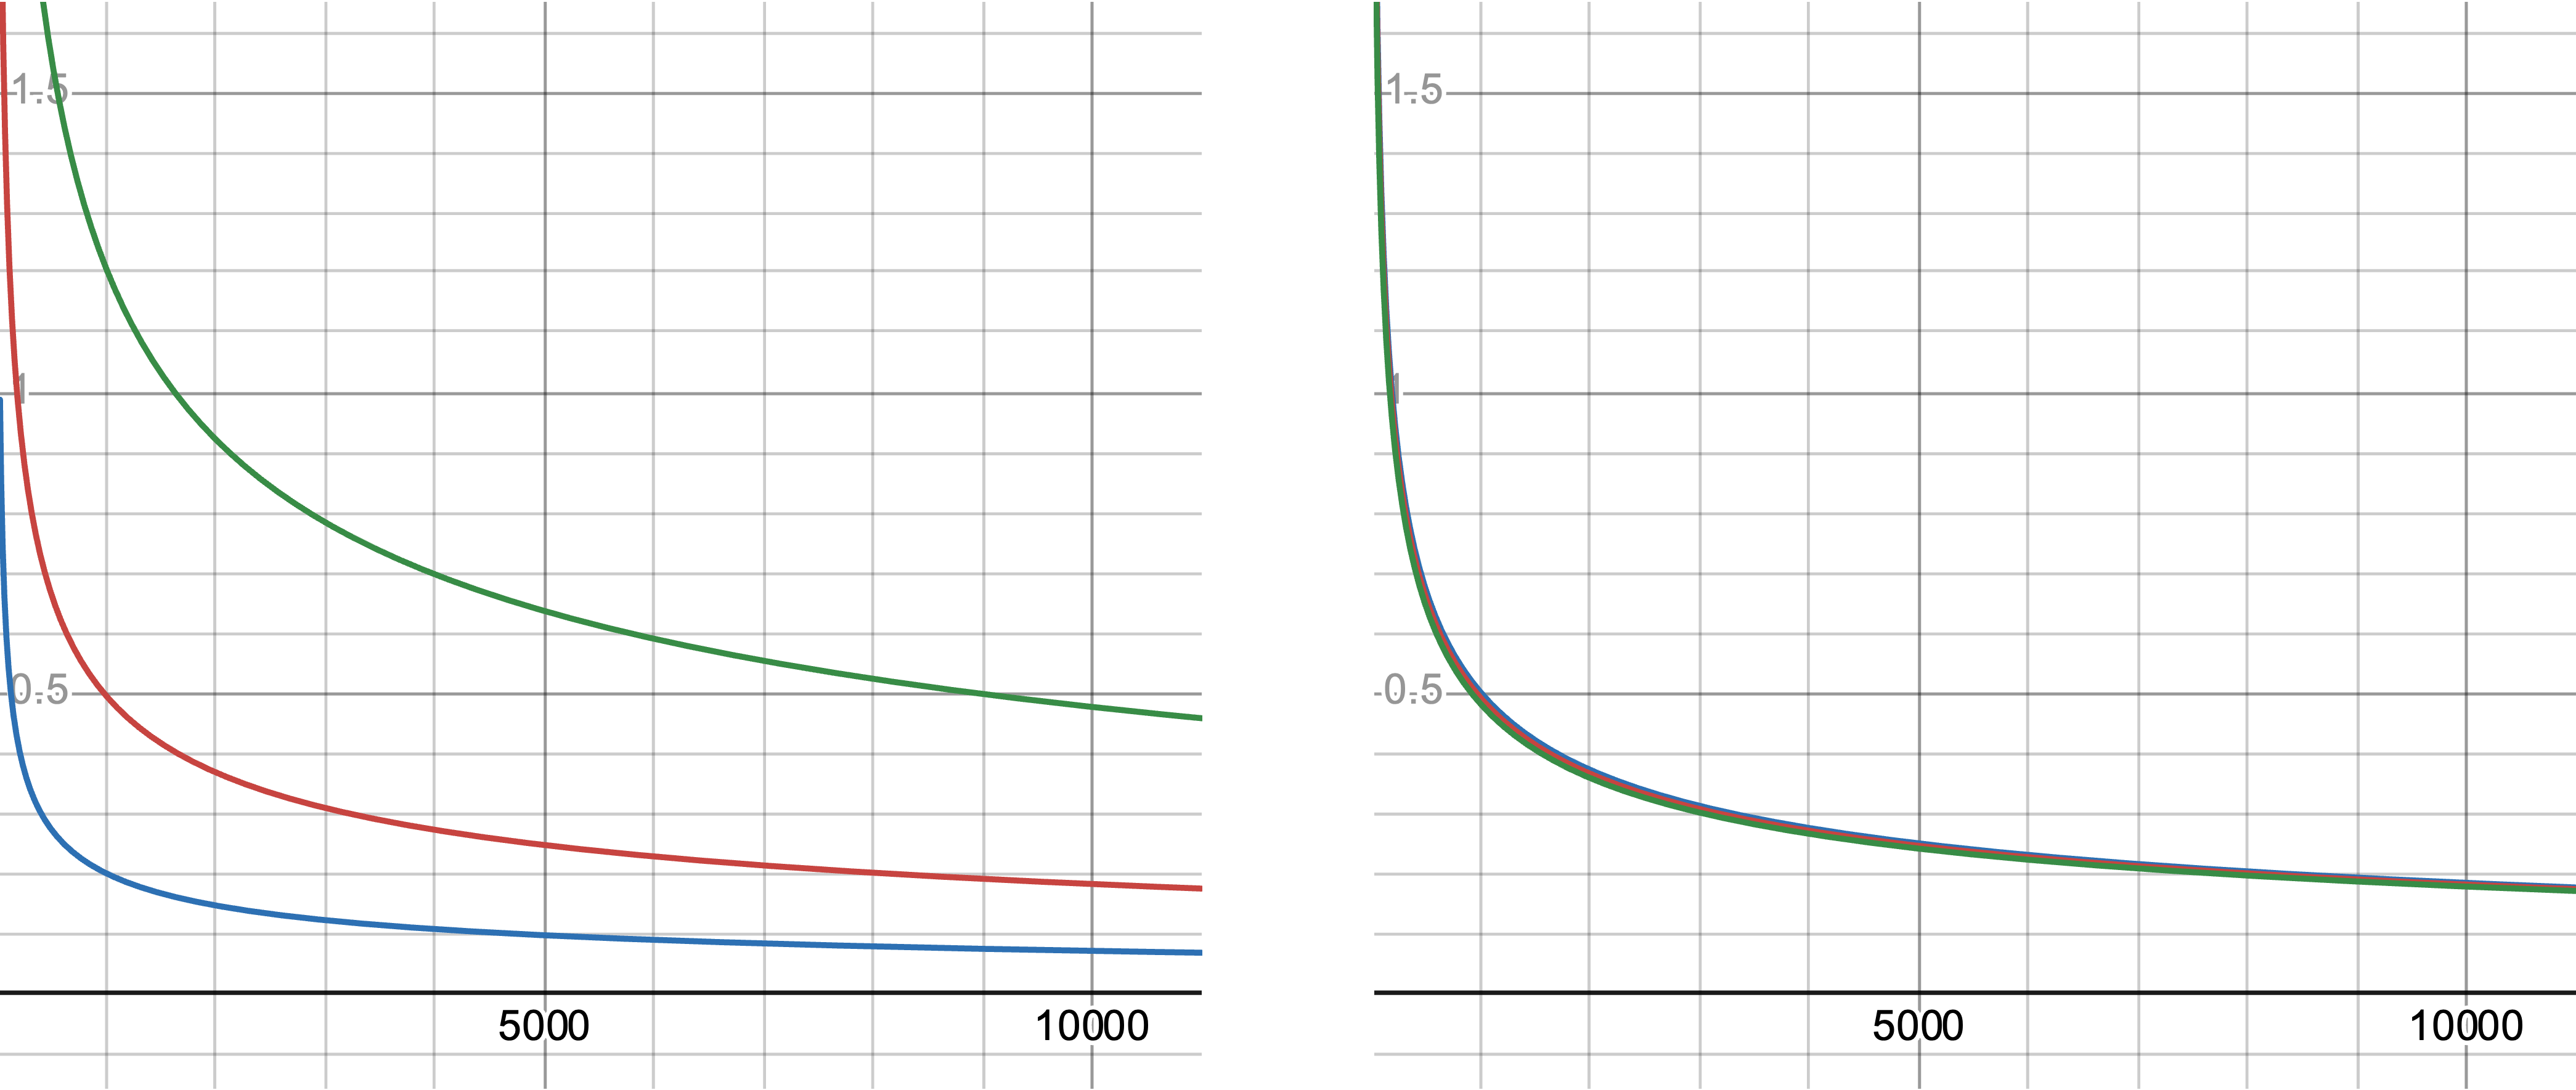
\includegraphics[width=15cm]{other/vc-inequality}
    \caption{%
         The bound provided by the VC inequality (Corollary \ref{cor: VC inequality}) depends much more on the VC dimension $V_{\mathcal{A}}$ and the number of samples $n$ than it does on the level of confidence $1 - \delta$. \textbf{Left}, illustration of the upper bound for sample size $n$ and VC dimension $1$ (\textcolor{desmos-blue}{\textbf{blue}}), $10$ (\textcolor{desmos-red}{\textbf{red}}), and $100$ (\textcolor{desmos-green}{\textbf{green}}). \textbf{Right}, illustration of the upper bound for sample size $n$ and confidence $1 - \delta$ set to $0.99$ (\textcolor{desmos-blue}{\textbf{blue}}), $0.9$ (\textcolor{desmos-red}{\textbf{red}}), and $0.5$ (\textcolor{desmos-green}{\textbf{green}}). \\
        \indent\emph{Note}. Created with the \href{https://www.desmos.com}{Desmos} Graphing Calculator. \href{https://creativecommons.org/licenses/by-nc-sa/4.0/}{CC BY-NC-SA 4.0}
    }
    \label{fig: VC inequality}
\end{figure}

Up to this point, we have shown that
\begin{equation}
\label{eq: precursor to VC inequality}
    \Exp[\sup_{A \in \mathcal{A}} \abs{\mu_n(A) - \mu(A)}] \leq 2 \mathfrak{R}_n(\mathcal{A}) \leq 2 \sqrt{\frac{2 \log(2 \mathcal{S}_{\mathcal{A}}(n))}{n}}.
\end{equation}
Note that this bound would not be informative (in the sense that it does not imply convergence of the uniform deviations to zero as the sample size $n$ goes to infinity) if the shatter coefficients $\mathcal{S}_{\mathcal{A}}(n)$ were exponential in $n$. For example, if $\mathcal{S}_{\mathcal{A}}(n) = 2^n$ for $n \leq V_{\mathcal{A}}$ and $\mathcal{S}_{\mathcal{A}}(n) = 2^n - 1$ for all $n > V_{\mathcal{A}}$, the RHS of \eqref{eq: precursor to VC inequality} would be greater than $2$ for all $n$. The VC inequality suggests that this cannot be the case, and indeed, if the VC dimension of a family of sets is \emph{finite}, the shatter coefficients of $\mathcal{A}$ can be at most \emph{polynomial} in $n$. This result is known as the Sauer-Shelah lemma:

\begin{lemma}[Sauer-Shelah]
\label{lem: sauer-shelah}
For a family of sets $\mathcal{A}$ with \emph{finite} VC dimension $V_{\mathcal{A}}$, the shatter coefficients satisfy
\[
    \mathcal{S}_{\mathcal{A}}(n) \leq \sum_{k=0}^{V_{\mathcal{A}}} \binom{n}{k}, \quad n \in \N.
\]
In particular,
\[
    \mathcal{S}_{\mathcal{A}}(n) \leq \left(\frac{\e n}{V_{\mathcal{A}}}\right)^{V_{\mathcal{A}}}, \quad n > 2 V_{\mathcal{A}}.
\]
\end{lemma}

For a proof of this result, we refer the reader to Theorem 13.2 and Theorem 13.3 in \cite[pp.~216--218]{devroye1996probabilistic}. Replacing $\mathcal{S}_{\mathcal{A}}(n)$ with $(\e n / V_{\mathcal{A}})^{V_{\mathcal{A}}}$ in \eqref{eq: precursor to VC inequality}---and observing that $\log(2x^n) \leq n \log(2x)$ holds for $n \in \N$ and $x > 0$---yields the VC inequality stated in Theorem \ref{thm: VC inequality}.

Recall that, using the bounded differences inequality (Theorem \ref{thm: bounded differences inequality}), we had shown that the bound
\[
    \sup_{A \in \mathcal{A}} \abs{\mu_n(A) - \mu(A)} < \Exp[\sup_{A \in \mathcal{A}} \abs{\mu_n(A) - \mu(A)}] + \sqrt{\frac{\log(\delta^{-1})}{2n}}
\]
holds with probability at least $1 - \delta$. Hence, we conclude:

\begin{corollary}[VC Inequality]
\label{cor: VC inequality}
For $n > 2 V_{\mathcal{A}}$ and a family of sets $\mathcal{A}$ with finite VC dimension $V_{\mathcal{A}}$, the upper bound
\[
    \sup_{A \in \mathcal{A}} \abs{\mu_n(A) - \mu(A)} < 2 \sqrt{\frac{2 V_{\mathcal{A}} \log(2 \e n / V_{\mathcal{A}})}{n}} + \sqrt{\frac{\log(\delta^{-1})}{2n}}
\]
holds with probability at least $1 - \delta$.
\end{corollary}

The upper bound provided by Corollary \ref{cor: VC inequality} is mostly driven by the number of samples $n$ and the VC dimension $V_{\mathcal{A}}$ of the family of sets $\mathcal{A}$. In contrast, the desired level of confidence $1 - \delta$ does not have much of an impact (see Figure \ref{fig: VC inequality}). For example, given a family $\mathcal{A}$ with VC dimension $V_{\mathcal{A}} = 4$, to guarantee an upper bound of $0.2$ with confidence $1 - \delta = 0.9$, we would need to observe $n = 3319$ samples. To increase the confidence we have in this bound from $0.9$ to $0.99$, we would only need to observe an additional $192$ samples. However, if the family $\mathcal{A}$ is slightly more complex in that it has VC dimension $5$ instead, we would have to observe an additional $769$ samples to guarantee the initial bound of $0.2$ with the same confidence (i.e., $1 - \delta = 0.9$). An interactive demo illustrating the bound's dependence on $V_{\mathcal{A}}$ and $\delta$ can be found at \url{https://www.desmos.com/calculator/fnfw9imfz1}.
